\chapter{Results and Discussions}
% The results and discussion for each solution considers the time taken for
% operations to complete on each of the entities  as described in the University
% example adopted for the experiments.

Performance of database systems is commonly measured in terms of the
\textit{Response time} and \textit{Throughput}(\todo{cite Demurjian, Berkely}).
Response time refers to the time  a database system takes to process an
operation and produce results to the end user . Measuring response time for a
database operation is similar to a black-box evaluation because it is measured 
without considering the internal functioning  of the database system. According
to (\todo{cite Demurjian}) such an evaluation is ideal for a complete database
system to measure its performance and to give the users details about its 
efficiency and speed in performing operations. In this thesis, response time and
throughput are the measures used to gauge the performance of Cassandra
while referential integrity validation is implemented using the \ac{API}.

Response time for each of the  operations that trigger such a validation from
all the solutions are measured during the experiments. This included the
time involved to access and retrieve metadata for the entities and also the time for
validating referential integrity by the \texttt{ValidationHandler}. The response
time of Cassandra when such validations are not in place is also measured and considered as a
baseline with which to analyse the solutions. Such a comparison  determines the degree of
change in speed of Cassandra when such overheads are introduced and gives 
users useful information about how each solution affects the performance of
the database system.

The second performance measure used is \textit{Throughput} which
is another classical and commonly used measure of database performance
(\todo{cite BerkleyDB}).
Throughput measures the number of operations processed by the database system in a unit of
time. In the experiments the throughput for all the operations
triggering referential integrity validation across all solutions is measured
as operations per second.
A single operation stands for each time an entity is inserted or updated or
deleted. 
% For example, inserting 1000 students means that 1000 \texttt{insert}
% operations are processed by Cassandra. 
Note that only the operations that
introduce the referential integrity validation in Cassandra is measured and thus
\texttt{read} operations are not measured in terms of response time or
throughput.
% These operations
% which trigger referential
% integrity validation for an entity
% namely the \texttt{insert}, \texttt{update}, \texttt{delete} operations are
% were measured in terms of the throughput in the experiments. Throughout commonly
% referes to the number of operations performed

It has to be noted that the operations are prone to  external factors like
network latency, bandwidth, network routing, network workload among others which
typically affect a network consisting of several machines and users. This is
because the Cassandra cluster used in the experiments is deployed over a
network that is used by many users concurrently thus exposing the operations to
such factors. Identifying such factors and analysing them is beyond the scope of
this thesis and the analysis is strictly in terms of how the metadata storage
and referential integrity validation affects Cassandra's performance.

 The results from the experiments were used to
analyse the performance of the four solutions with respect to  response
time and throughput and this is discussed in the following sections.
Section~\ref{sr:baseline} presents the results for the baseline experiment where 
% no referential validation checks are implemented
% and t
the operations performed on the entities are just as it would be performed in
Cassandra. Section~\ref{sr:insert} analyses the results of all the solutions
for the \texttt{insert} operation. Section~\ref{sr:update} presents the analysis
for the \texttt{update} operation for all the solutions. Section~\ref{sr:delete}
discusses the results of the solutions for the \texttt{delete} operation. 


\section{Baseline}\label{sr:baseline}
The performance of Cassandra when referential
integrity validation is introduced using any of the solutions is compared with a
a base experiment where the operations on the entities do not trigger any
such validations. Such a baseline is useful to determine the
performance of the database system when validations are imposed using the
\ac{API} and to analyse the performance of the solutions.
% baseline experiment has no referential integrity validation introduced and
In the baseline experiment, the operations on the entities represent how
data is inserted into Cassandra without referential integrity validations. The
results in terms of response time for the baseline experiment is presented as
a bar-plot in Figure~\ref{fr:Solution0-barplot}. The analysis of
the performance of each operation on an entity is discussed as follows.
% The results are analysed in the
% following 

% The factors measured were the time involved to complete each operation for every
% entity, where the operations considered were the ones that invoked referential
% integrity validation, namely, \texttt{insert}, \texttt{update} and
% \texttt{delete}. These were measured for the entities in the University example,
% namely \texttt{Student}, \texttt{Course} and \texttt{Enrolment}.
% The results are plotted as a histogram in Figure~\ref{}
	
\begin{figure}[h] \centering
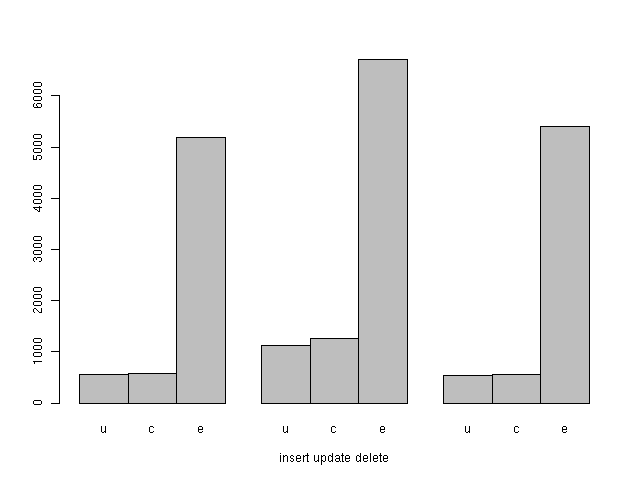
\includegraphics[width=.8\textwidth]{./figure/result/Solution0-barplot.png}
		\caption{Baseline}\label{fr:Solution0-barplot}
	\end{figure}
	
% Present results.
% 	The potential reasons for the variance of time for the completion of each
% 	operations on the different entities are summarised next.
	\begin{description}
	\item[Insert] The results from the baseline experiment show that the time for
	inserting entities into the \texttt{Student} and \texttt{Course} column families 
	are similar. This is because the number of entities inserted into these
	column families are exactly the same.
% 	\texttt{1000} instances of \texttt{Student} and \texttt{Course} are inserted
% 	into the respective column families in the baseline experiment. 
	The time taken
	to insert the \texttt{Enrolment} entities into the \texttt{Enrolment} column family
	is higher by approximately \texttt{4} seconds. This is because
	\texttt{Enrolment} has more entities than the other column families, to be
	specific it has \texttt{10,000} instances which is 10 times more entities than
	\texttt{Student} and \texttt{Course}.
% 	Hence, the \texttt{insert} operation takes more time to insert entities into \texttt{Enrolment} column family, especially considering its
% 	replication across \texttt{10} nodes, which would add to the time in
% 	completing the operation.
	
	\item[Update] The time for updating the primary keys in \texttt{Student} and
	\texttt{Course} are comparable to each other. Although the number of entities
	updated are the same, the small difference is owing to external variables
	(e.g. network latency, high network traffic). Similar to the \texttt{insert}
	operation, updating the \texttt{Enrolment} entities takes significantly more
	time, which is again due to the higher number of entities held within this
	column family. 
	
	The  response time of the \texttt{update} operation on
	\texttt{Enrolment} is higher when compared to the response  time of
	\texttt{insert} operation on the same. This is mainly due to the additional
	computational resources consumed to ensure the existence of an entity before
	updating it to new values.
	
	\item[Delete] The time involved for completion of the \texttt{delete} operation
	on all the entities from \texttt{Student} and \texttt{Course} column families
	are similar to each other owing to the same number of entities. The time
	involved for the \texttt{delete} operation to delete all the entities in
	\texttt{Enrolment} is higher just as in other operations. This is again due to
	the larger number of entities present in \texttt{Enrolment}.
	
	Performance of the \texttt{delete} operation is similar to the\texttt{insert}
	operation in terms of time taken for completion and the processes involved. This
	means that unlike \texttt{update} both \texttt{delete} and \texttt{insert} do
	not involve additional operations and simply adds or removes entities from the
	column families. It should also be noted that external factors affect the
	performance of the operations.
	
	\end{description} 

	
	
% 	Explain Insert. Why student and course similar. Why enrolment much higher.
% 	

	In general, all the operations take more time to complete on the
	\texttt{Enrolment} column family due to its larger number of entities 
	when compared to \texttt{Student} and \texttt{Course} column families. The
	\texttt{update} operation consumes more time due to the additional search
	involved to locate the previous state of the entity prior to updating it to new
	values. Notice that the time involved to complete \texttt{insert} and
	\texttt{delete} entities form all the three column families are similar.
	
	The following sections analyse the performance of each solution  in
	terms of how its referential integrity validation in each of the
	\texttt{insert}, \texttt{update} and \texttt{delete} operation and its
	metadata storage affect the performance.
	
\section{Insert}\label{sr:insert}
An \texttt{insert} operation triggers a referential integrity validation
whenever a child entity containing foreign keys is inserted where the
\texttt{ValidationHandler} validates that the foreign keys exist as primary keys in the parent
entities. 
% This dependency information is retrieved from the metadata saved in
% each solutions. 
In the experiments, the time taken to insert all the
entities are recorded thus also measuring the time involved for validating
referential integrity for each entity. Across all the solutions in the
experiments, the \texttt{insert} operation triggers such a validation when the
\texttt{Enrolment} entities are inserted since it is a child entity containing
foreign keys of \texttt{Student} and \texttt{Course} entities.
%  As mentioned in
% Section~\ref{s:exp:setup} the number of entities inserted into the
% \texttt{Enrolment} column family is the same for all solutions and the baseline
% experiment.
% Despite the same number of entities and similar validation performed, 
The response time and throughout of the \texttt{insert} operation in all the
solutions and the baseline experiment are plotted in
Figure~\ref{fr:insert-result}.
% 	\begin{figure}[H] \centering
% 	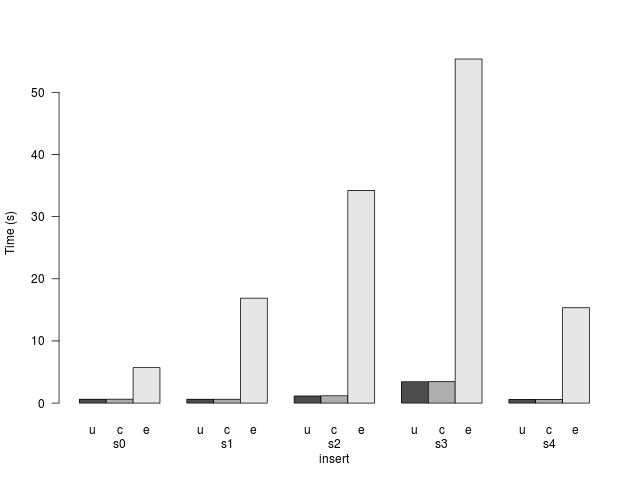
\includegraphics[width=.8\textwidth]{./figure/result/op-insert-barplot.png}
% 		\caption{}\label{fr:response-insert}
% 	\end{figure}
	
	
	
	
	
	
	
	
The results of all the solutions as seen in Figure~\ref{fr:insert-result} with
respect to response time  is discussed as follows based on the different
entities on which the \texttt{insert} operation is applied.
\subsection{Response Time}
\begin{itemize}
  \item The results show that the response time of all
  the solutions to insert entities into \texttt{Student} and \texttt{Course}
  column families is similar and always lesser than 5 seconds. This is because
  no referential integrity validation is invoked when parent entities are
  inserted as these do not contain any foreign keys. Note that the metadata for
  any entity is accessed and checked by the \texttt{ValidationHandler}
  to determine if it has dependencies or not. It is during this
  check that it is determined if an entity is a parent or child. 
  So across all solutions even when parent entities \texttt{Student} and
  \texttt{Course} are inserted their metadata is accessed.
  
  Solutions~1, 2  and 4 have approximately similar response times since the metadata 
  access for these solutions are easier as metadata is a part of the entity and 
  no additional connection to a metadata column family is required. Solution~3
  takes slightly longer than the rest of the solutions and this is because of the way
  the metadata is accessed for the entities in this solution. 
% irrespective of whether an entity is a parent or child the
% \texttt{ValidationHandler} performs the same check the metedata of the entity
% for all the solutions. It is when this check is made it is clear if the entity
% is a parent or child. 
  In this solution accessing the metadata for every 
  \texttt{Student} and \texttt{Course} entity causes the slower
  response time since a different \texttt{Metadata} column family has to be
  accessed using the connection object. This is because metadata is not cached
  for re-use in this solution. Unlike this, Solution~4 caches  metadata for
  entities and re-uses it thus saving time by not having to access a separate
  column family for each entity insertion.
  
  When compared to the baseline experiment the insertion of parent entities
  in all the solutions, except Solution~3, take similar response times despite
  the initial metadata access. Solution~3 takes only a few seconds
  longer to complete the operation when compared to the baseline.
  


  \item The response time involved for inserting the \texttt{Enrolment}
  entities differs across solutions. Since these entities have existing \ac{FK}
  constraints in their metadata indicating they are dependent on a parent
  entity, referential integrity validations are triggered. The results in
  Figure~\ref{fr:insert-result} show that Solutions~1 and 4 take approximately 15 seconds to
  insert  \texttt{Enrolment}entities and take the least time when compared
  to the other solutions.  Solution~2 takes lesser than 35 seconds while
  Solution~3 takes longer than the rest of the solutions 
  This is mainly due to the way metadata is accessed and read from  a different
  \texttt{Metadata} column family in this solution. In the rest of the solutions the 
  metadata is either a part of the entity, making the access easier or it is
  cached as in Solution~4 thus requiring no extra connections to a column family. 
  
  As seen in the baseline experiment inserting \texttt{Enrolment} entities  has
  a higher response time in the solutions. But the response time for this
  operation on \texttt{Enrolment} is higher in the solutions when compared to
  the baseline experiment. This means that referential integrity validation in
  each solution increases the response time slightly, depending on the way the
  metadata is accessed for the entities in the solutions. Moreover, the entities
  inserted into the \texttt{Enrolment} column family is ten times more than the
  other column families.
% The validation involves accessing the columns of the  column family in this
% solution to get each value of the constraint.
\end{itemize}

Generally, the response time for inserting child entities is higher across the
solutions when compared to the response time for inserting parent entities. In
the baseline experiment this was solely because of the larger number of entities
in the child entity class, while in the solutions it was due to the referential
validation triggered while inserting child entities and also the larger number
of entities. Inserting parent entities is similar in the baseline
experiment and the solutions despite the metadata access present in the
solutions. This is so because no additional validations are triggered in the
solutions. 


\subsection{Throughput}

To summarise this operation, the results show that Solutions~1 and 4 perform
similarly with respect to inserting child and parent entities and are faster
 than the rest of the solutions while Solution~3 is the slowest for both the
 cases. the different response times for the solutions are owing to the
 different styles of metadata storage as explained previously.

%  It can be that the response time  
%  On the other hand, Solution~4 caches the metadata information for entities and
%  does not need to connect to the metadata column family each time any operaion
%  is triggered on an entity. Solutions~1 and 2 take approximately the same time
%  and the metadata access for these solutions are easier as it comes as a part of
%  the entity and no additional connetion to the metadata is required. 
%  
% 
% On the other hand the time consumed to insert \texttt{Enrolment} entities varies
% across the solutions since there is referential integrity validation where
% metadata constraints are read and validated.

		
% Performing the \texttt{insert} operation for the 10000 entities in
% \texttt{Enrolment} is thus more time consuming for all the solutions when
% compared to inserting entities into other column families and this is similar to
% the baseline experiment where inserting \texttt{Enrolment} entities was more
% time consuming.
% However in the solutions, the time taken to insert entities into
% \texttt{Enrolment} is higher when compared to the same in the baseline tests and
% this is  due to the referential validation that is triggered while inserting
% child entities in the solutions. 
\newpage

\newcommand{\Width}{.8\textwidth}
	\begin{figure}[H] \label{fr:insert-result}
		\centering
		\subfigure[Response Time]{
			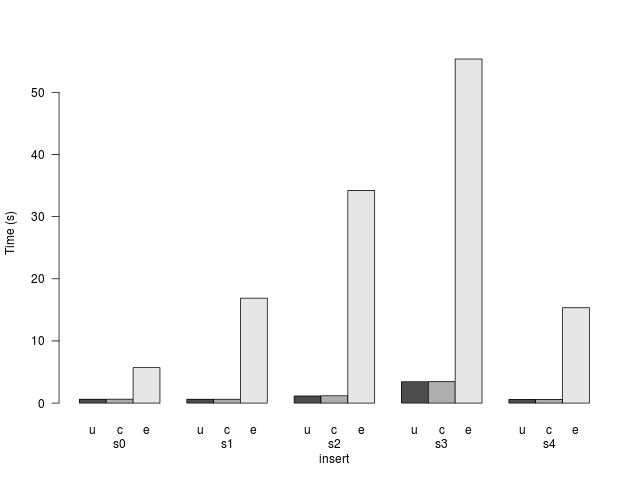
\includegraphics[width=\Width]{./figure/result/op-insert-barplot.png}
% 			\caption{Response Time for \texttt{insert}}\label{fr:response-insert}
		}
		\subfigure[throughput]{
			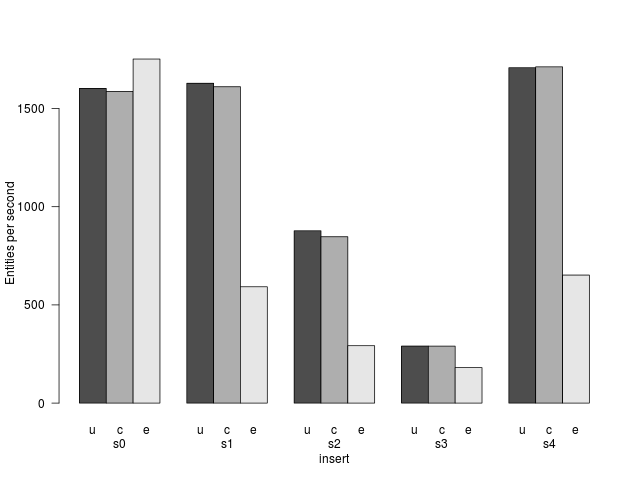
\includegraphics[width=\Width]{./figure/result/th-insert-barplot.png}
% 			\caption{Throughput}\label{fr:through-insert}
		} 
	\caption{Response time and Throughput of \texttt{insert} operation}
	\end{figure}

\section{Update}\label{sr:update}
In all the solutions, the \texttt{update} operation triggers a referential
integrity validation whenever an entity is updated with new values. 
% Moreover,
% data manipulation rules are also applied which specifies whether the \texttt{update} is a
% \texttt{Cascade} or \texttt{NoDelete}. 
The \texttt{ValidationHandler} in all the
solutions perform these validations and accesses metadata and its various parts
to determine whether referential integrity is violated or not. This is
unlike the baseline experiment where  no referential integrity
validations  are performed and entities are updated without
checking its correctness or validity. 

In all the solutions the time taken to update the primary keys in
\texttt{Student} and \texttt{Course} column families and the time taken to
update the foreign key \texttt{CourseId} in \texttt{Enrolment} is measured
in terms of response time and throughput. The
results are presented in Figure~\ref{fr:update-result} and the performance of
the solutions in an \texttt{update} is discussed next.

	\begin{figure}[h] \label{fr:update-result}
		\centering
		\subfigure[Response Time]{
			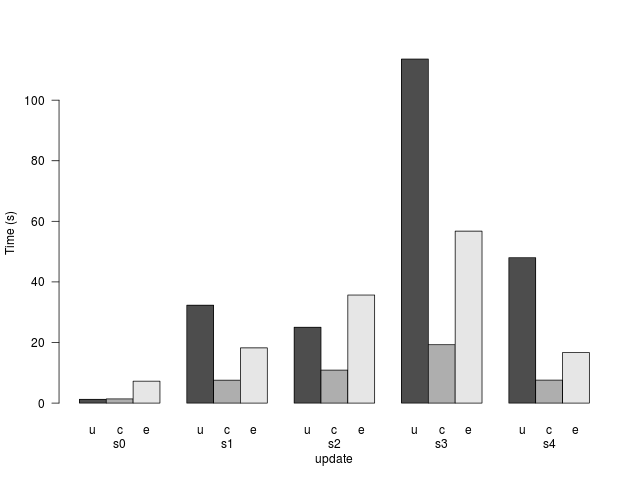
\includegraphics[width=\Width]{./figure/result/op-update-barplot.png}
% 			\caption{Response Time for \texttt{insert}}\label{fr:response-insert}
		}
		\subfigure[Throughput]{
			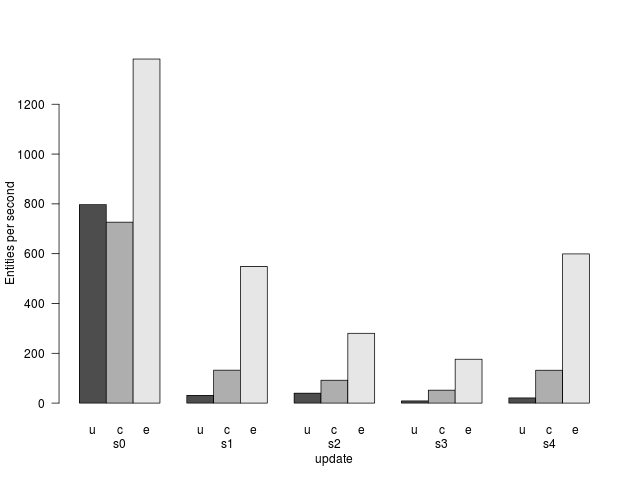
\includegraphics[width=\Width]{./figure/result/th-update-barplot.png}
% 			\caption{Throughput}\label{fr:through-insert}
		} 
	\caption{Response time and Throughput of \texttt{insert} operation}
	\end{figure}
	
	\subsection{Response Time}
	The response time of the solutions based on the results fro the experiments are
	analysed and is categorised on the different cases applicable in the
	\texttt{update} operation. The different cases are a cascaded
	and \texttt{NoDelete} \texttt{update} operations on primary keys and 
	the foreign key updates in child entities.
	
	
	\begin{itemize}
	  \item The \texttt{update} operation on \texttt{Student} entities is
	  cascaded since the \texttt{DeleteRule} for \texttt{Student} is
	  \texttt{Cascade} . Note that for the cascaded \texttt{update} operation
	  the dependent values in \texttt{Enrolment} is also updated, 
	  which incurs additional time for this operation to complete.
% 	  Updating \texttt{Student} entities involve cascading
% 	  the changes within the child entity \texttt{Enrolment}.
% 	%  while updating \texttt{Course} throws an
	% exception since \texttt{course} entities have a \texttt{NoDelete} manipulation
	% rule in its metadata, thus preventing the \texttt{update}. 
	The results in Figure~\ref{fr:update-result} show that all the solutions have
	different response times for updating \texttt{Student} entities.
	Solution~2 takes the least time to perform the updates when compared to the
	other solutions while Solution~1 takes approximately 10 seconds more than
	Solution~2.(\todo{check update of Sol2}) Solution~3 has the highest response
	time of 100 seconds and this is because for each \texttt{update} operation
	on \texttt{Student} entities, the metadata column family in this solution is
	accessed and the metadata is processed each time by the
	\texttt{ValidationHandler} to validate referential integrity. Solution~4 is
	faster than Solution~3 mainly because it caches the metadata for the entity
	class and uses the cached metadata for all the entities of the entity class.
	This helps in saving time as \texttt{ValidationHandler} does not have to access
	a separate column family for each operation.  
	% slightly more than 25 seconds to
	% perform a cascaded \texttt{update} for \texttt{Student} entities.
	But Solution~4 takes longer than Solutions~1 and 2 because despite the cached
	metadata it has to initially fetch the metadata from an external location unlike
	the latter solutions. 
	% olution~2 takes slightly more than 20 seconds and takes
	% lesser time than other solutions, while Solution~3 takes the most time of more than 60 seconds. 
	All the solutions takes more time to insert \texttt{Student} entities when compared to
	the baseline due to the referential integrity validation and the cascaded
	operations, which additionally accesses \texttt{Enrolment} to complete the
	\texttt{update} operation. The difference in response time when referential
	integrity validation is in place and when it is not in the baseline experiment
	ranges from more than 20 seconds to above 100 seconds.
	
	  \item Updating \texttt{Course} entities involves identifying the metadata
	constraints and raising an exception due to the \texttt{NoDelete} rule applicable for every
	\texttt{Course} entity. From the
	results in Figures~\ref{fr:update-result} it can inferred that both Solutions~1 and 4 take
	the least time amongst all solutions to insert \texttt{Course} entities. These
	solutions take least time since for the former the metadata is easily accessed
	being a part of the entity thus not requiring additional accessing time.
	Solution~4 access the entity metadata from the cached metadata maintained in
	this solution, making it faster to fetch the metadata for all entities of a
	particular entity class. 
% 	where Solution~1 takes less than 5 seconds and
% 	Solution~4 close to it.
	Solution~2 is not far behind form these solutions and
	takes slightly more than 5 seconds. This is because in Solution~2 the metadata
	is accessed for each entity after searching for the top row incurring some
	additional time every time an entity is updated. Solution~3 takes nearly twice
	the amount of time than the rest of the solutions for this operation. Just as
	in updating \texttt{Student} entities this is due to the separate access
	required to the \texttt{Metadata} column family and identifying the appropriate constraints for an entity class in it. 
	
	When compared to the baseline, updating \texttt{Course} takes more time in all
	solutions since  validations are triggered and  exceptions are raised unlike
	the baseline. The only difference between this operation in the solutions and the
	baseline experiment is the time involved in accessing the metadata and
	determining the \texttt{DeleteRule} and handling the exceptions.
	
	\item When \texttt{Enrolment} entities are  updated the changes are applied
	only within the
	\texttt{Enrolment} column family although \texttt{Student} and
	\texttt{Course} column families are accessed to ensure the new
	foreign keys exist. The results in Figure~\ref{fr:update-result} show that
	Solutions~1 and 4 almost take almost the same time. This is similar to the
	\texttt{update} on \texttt{course} entities and is because of the way the
	metadata is accessed and used by the \texttt{ValidationHandler}. 
	Solution~2 takes slightly more than Solutions~1 and 4 because of the way it
	has to search for the top row to identify the entities metadata each time.
	As seen in previous cases, Solution~3 takes the highest time and this is owing
	to the separate access to \texttt{Metadata}. column family.
	
	When compared to the baseline experiment, the solutions are slower because
	parent column families are accessed always  to check the existence of the new
	values in every validation by the \texttt{ValidationHandler}. 
	\end{itemize}
	
Generally, in all the solutions updating the \texttt{Course} entities take the
least time when compared to updating \texttt{Student} or \texttt{Course}
entities. This is because although \texttt{update} on \texttt{Course} entities trigger
validation, the entities are not updated and neither are any cascade operations
performed.
The time involved in updating \texttt{Students} is higher than updating the
\texttt{Enrolment} entities due to the cascading operations  and
the changes made in child column families.
Moreover for \texttt{update} on \texttt{Enrolment} the validation is limited to
accessing the parent entities to ensure the existence of the foreign keys.
The \texttt{update} on \texttt{Enrolment} takes more time than \texttt{update}
on \texttt{Course} since updating \texttt{Enrolment} involves changing the
values and accessing the parent entity classes for
validation unlike \texttt{update} on
\texttt{Course} where
validation takes place but no other column families are accessed nor are values
changed. 

	%		Take to Summary of Solutions
% 													Overall, it is clear that Solution~3 takes more time  to update all the
% 													different entities, while Solutions~1 takes the least time to update all the entities.
% 													Some cases of the \texttt{update} operations are similar in speed in both
% 													Solutions~1 and 4. Solution~2 is slower than Solutions~1 and 4 but faster than
% 													Solution~4.


% It is interesting to note that in 	Solution~2 the time for updating the
% \texttt{Enrolment} entities is more than updating \texttt{Student} entities
% unlike all the solutions. This is mainly because an \texttt{update} involves an
% \texttt{insert} and \texttt{delete} operation. It can be seen that this
% \texttt{update} on \texttt{Enrolment} is similar to the time taken to
% \texttt{insert} the \texttt{Enrolment} entities in this solution. The difference
% in the way metadata is stored and retrieved is also another cause for this
% anomaly and is further explained in Section~\ref{}.


\section{Delete}\label{sr:delete}
In all the solutions, the \texttt{delete} operation triggers a referential
integrity validation whenever a parent entity is deleted. Just as in an
\texttt{update}, a cascaded 
\texttt{delete} requires that dependent entities are removed from
\texttt{Enrolment}.
In all the solutions the time taken to delete the entities  are recorded and
experiments are designed to test every case of the \texttt{delete} operation.
This means that both cascaded deletes of \texttt{Student} entities and deletions
of
\texttt{Course} entities with no dependencies are tested. The results of the
experiment is presented in Figure~\ref{fr:delete-result}The performance of the
solutions in these different cases involved is discussed next.

	\begin{figure}[h] \label{fr:delete-result}
		\centering
		\subfigure[Response Time]{
			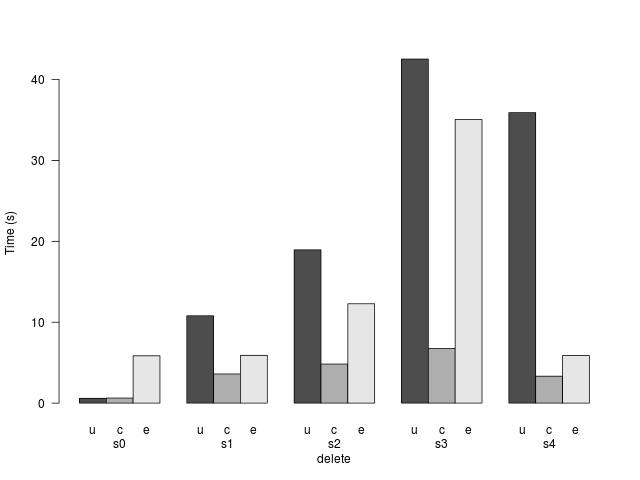
\includegraphics[width=\Width]{./figure/result/op-delete-barplot.png}
% 			\caption{Response Time for \texttt{insert}}\label{fr:response-insert}
		}
		\subfigure[Throughput]{
			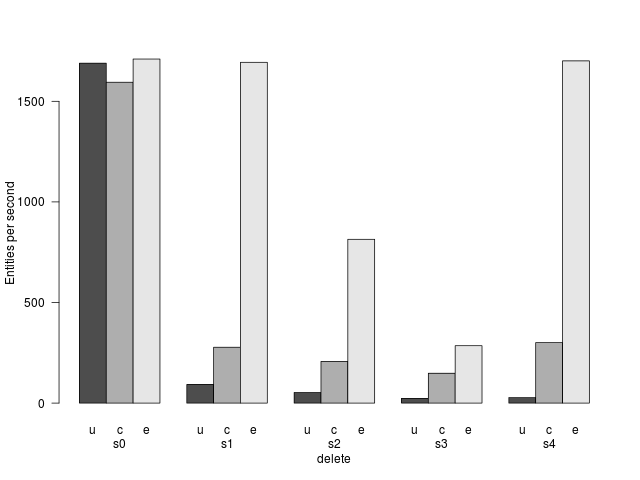
\includegraphics[width=\Width]{./figure/result/th-delete-barplot.png}
% 			\caption{Throughput}\label{fr:through-insert}
		} 
	\caption{Response time and Throughput of \texttt{delete} operation}
	\end{figure}

\begin{itemize}
  \item Deleting \texttt{Student} entities involved  deleting  the \texttt{Enrolment} 
  entities that had dependent foreign keys. Similar to the \texttt{update}
  operation, this meant some additional time to complete the operation.
%   This cascaded delete was determined
%   from the \texttt{DeleteRule} of the \ac{PK} constraint of \texttt{Student}
%   entities.
% this operation involved deleting \texttt{enrolment} entities that had the
%   \texttt{StudentId} of the \texttt{Student} entity marked for deltion as a
%   foreign key. 
%   In this case, the time measured involved the cascaded delete of
%   entities from \texttt{Enrolment} and then the deletion of the \texttt{Student}
%   entity from the \texttt{Student} column family. 
  From Figure~\ref{fr:delete-result}, it can be
  summarised that Solution~1 took the least amount of time with less than 10
  seconds and Solution~3 took more than 20 seconds to complete the cascaded
  deletion.When compared to the baseline, all the solutions take considerably
  longer to perform the \texttt{delete} on \texttt{Student} entities. This is
  because of the referential integrity validation and the cascaded operations.
  Like \texttt{update} this operation also accesses another column family to
  complete the operation.
  
  \item Deleting the \texttt{Course} entities also invoked referential
  integrity validation and despite its \texttt{NoDelete} rule, \texttt{Course}
  entities that had no current dependencies in \texttt{Enrolment} were deleted
  and the time measured. The results show that Solutions~1 and 4 take
  approximately 2 seconds while Solutions~2 and 3 take slightly less than 5
  seconds.When compared to the baseline this operation generally takes slightly
  longer. This is because prior to the deletion of the entities all solutions
  perform the validation and checks the metadata. The operation then deletes the
  entities when no child dependencies exist.
  
  \item Deleting \texttt{Enrolment} invokes no validation although the metadata
  is checked for the entity. Solutions~1 and 4 take slightly more than 5
  seconds to complete this operation while Solution~2 takes more than 10
  seconds. Solution~3 takes more than 20 seconds to complete the operation and
  is the longest when compared to the other solutions. When compared to the
  baseline, the solutions take longer to complete despite having no referential
  integrity constraints. This is because when the \texttt{delete} operation is
  invoked on \texttt{Enrolment} it is treated as any other entity and its
  metadata is accessed and \texttt{ValidationHandler} determines if any
  \ac{FK} constraints exist for it.
  
\end{itemize}

In general, deleting \texttt{Student} entities take the longest time in all the
solutions unlike the baseline. The time is higher due to the validation and the
cascaded operation which accesses another column family in the cluster. The
\texttt{delete} on \texttt{Enrolment} is lower than \texttt{delete} on
\texttt{Students} because \texttt{Enrolment} has no dependencies and the
validation involves checking whether it has any child dependent on it. Apart
form this metadata checking, the entities are deleted just as in the baseline.
The operation is shortest when \texttt{Course} entities are deleted and is
because similar to deleting \texttt{Enrolment} validation is performed and the
delete takes place. It takes lesser time than deleting \texttt{students} because
data in other column families are not accessed or changed. Although similar to
\texttt{delete} on \texttt{Enrolment}, \texttt{Course} takes lesser time due to
its lesser number of entities when compared to \texttt{Enrolment} entities which
is 10 times more.



% \newcommand{\Width}{.5\textwidth}
% 	Explain update. Student and course are similar, small difference to external
% 	variables (e.g. network latency). Same, enrolment is higher. Blame update
% 	higher times than insert due to additional computational resources spent
% 	ensuring the previous existence of the record before changing new values.
% 	
% 	Delete. Similar to insert. It does not require changing values, but just
% 	removing. However, notice that in average the differences between insert and
% 	delete are rather small, and both with respect to update are a bit bigger.

\begin{figure}
	\centering
	\subfigure[Solution1]{
	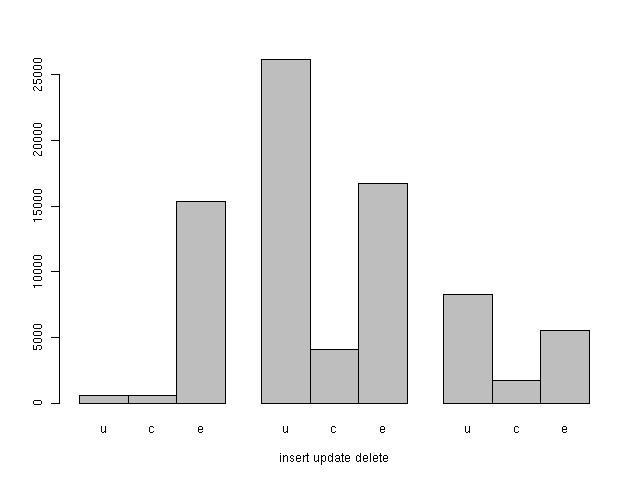
\includegraphics[width=\Width]{./figure/result/Solution1-barplot.png}
	}\subfigure[Solution2]{
	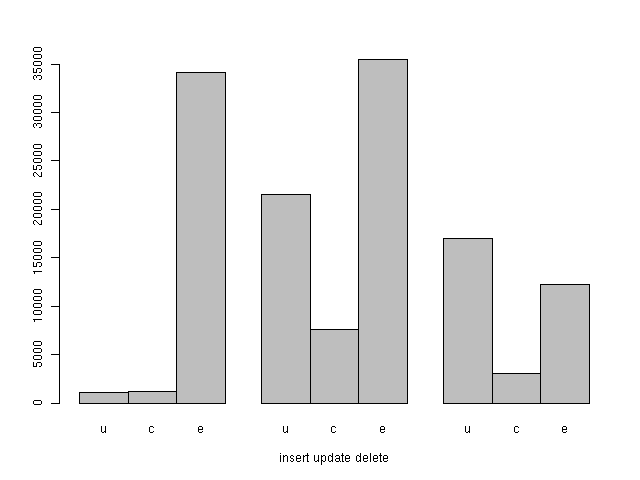
\includegraphics[width=\Width]{./figure/result/Solution2-barplot.png}
	}\\
	\subfigure[Solution3]{
	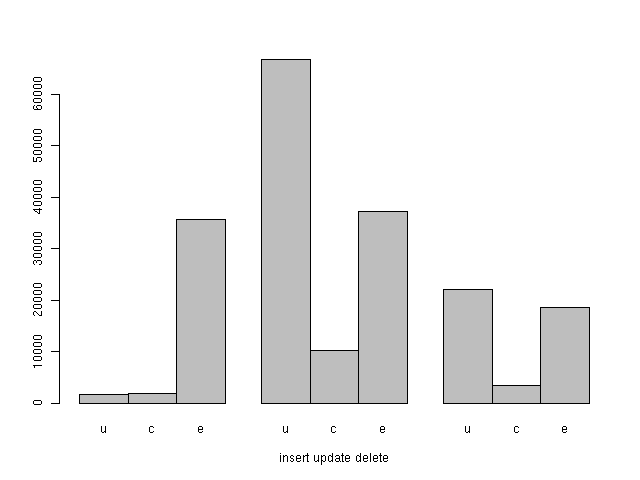
\includegraphics[width=\Width]{./figure/result/Solution3-barplot.png}
	}\subfigure[Solution4]{
	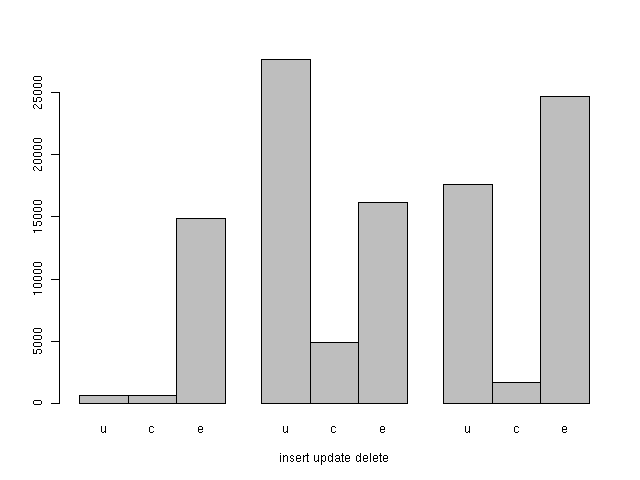
\includegraphics[width=\Width]{./figure/result/Solution4-barplot.png}
	}\\
	\subfigure[Baseline]{
	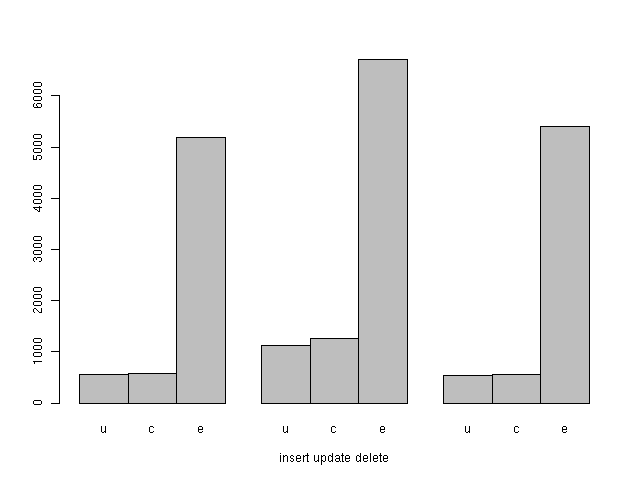
\includegraphics[width=\Width]{./figure/result/Solution0-barplot.png}
	}
\end{figure}


\renewcommand{\Width}{.6\textwidth}
\begin{figure}
	\centering
	\subfigure[User]{
	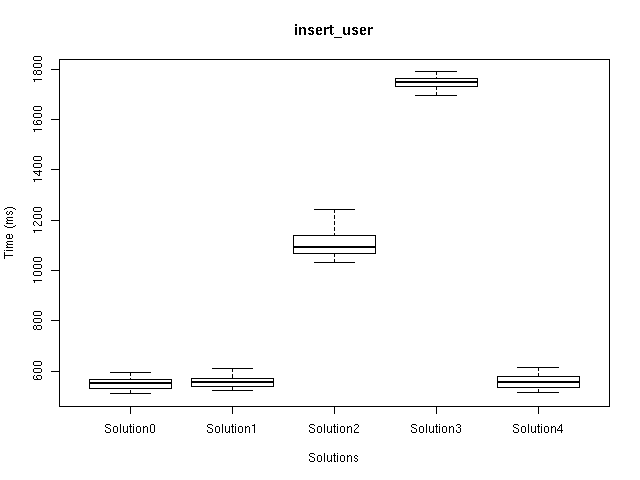
\includegraphics[width=\Width]{./figure/result/bp-insert_user.png}
	}
	\subfigure[Course]{
	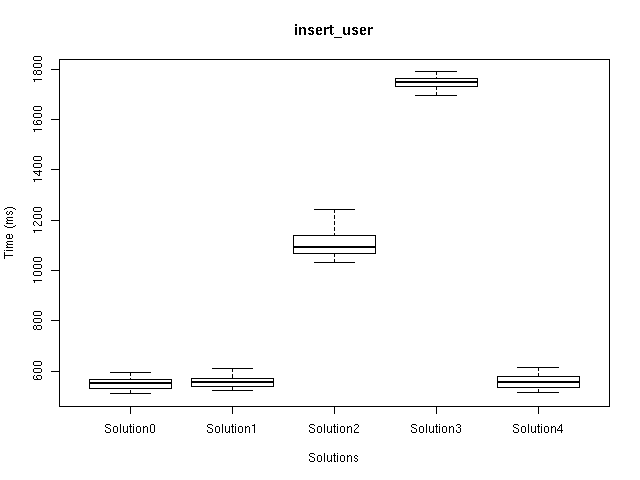
\includegraphics[width=\Width]{./figure/result/bp-insert_user.png}
	}
	\subfigure[Enrolment]{
	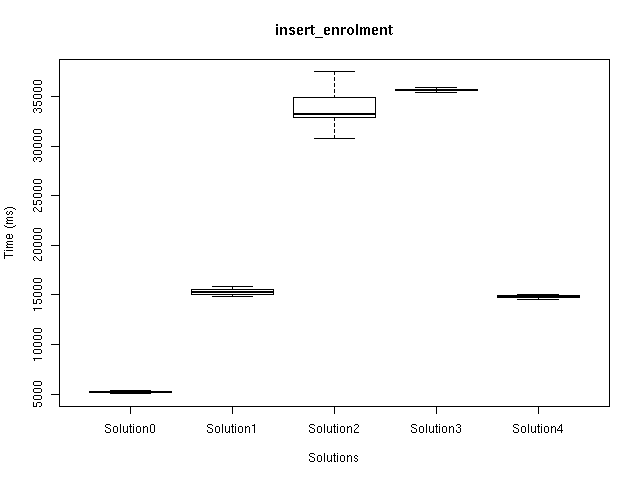
\includegraphics[width=\Width]{./figure/result/bp-insert_enrolment.png}
	}
	\caption{Insert}
\end{figure}


\begin{figure}
	\centering
	\subfigure[User]{
	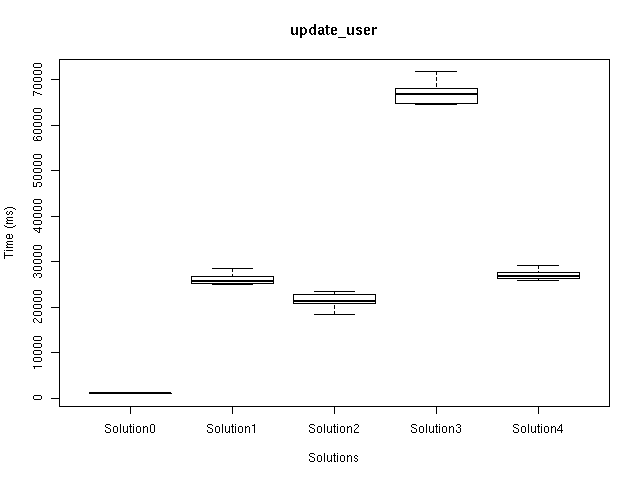
\includegraphics[width=\Width]{./figure/result/bp-update_user.png}
	}
	\subfigure[Course]{
	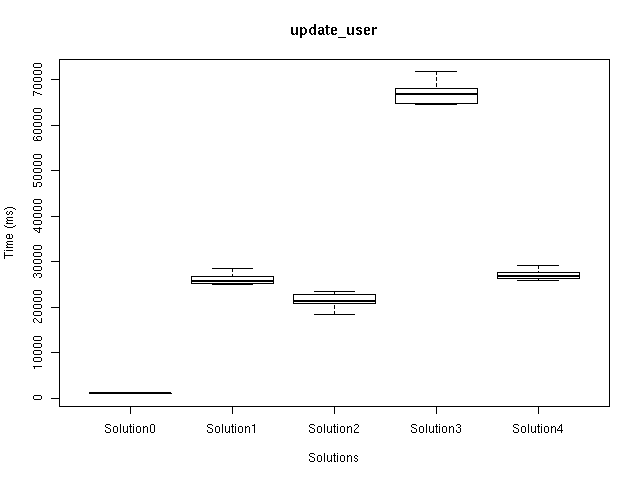
\includegraphics[width=\Width]{./figure/result/bp-update_user.png}
	}
	\subfigure[Enrolment]{
	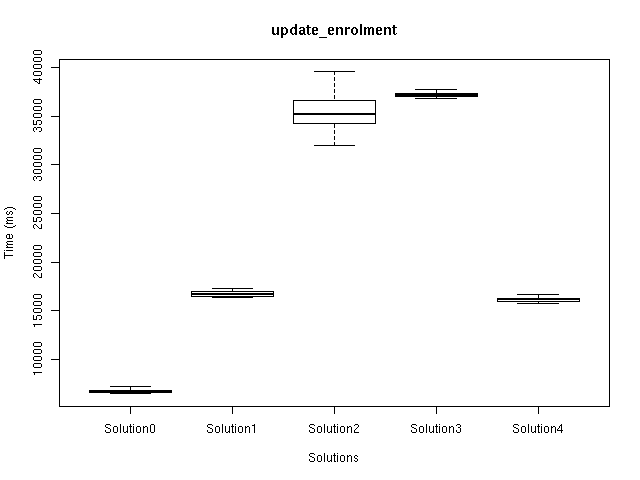
\includegraphics[width=\Width]{./figure/result/bp-update_enrolment.png}
	}
	\caption{Update}
\end{figure}


\begin{figure}
	\centering
	\subfigure[User]{
	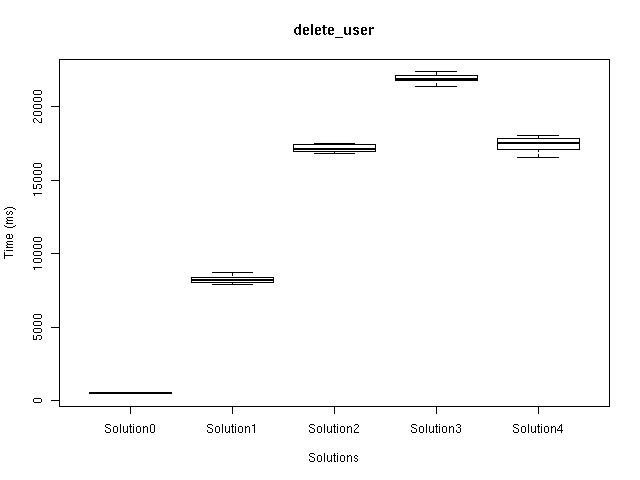
\includegraphics[width=\Width]{./figure/result/bp-delete_user.png}
	}
	\subfigure[Course]{
	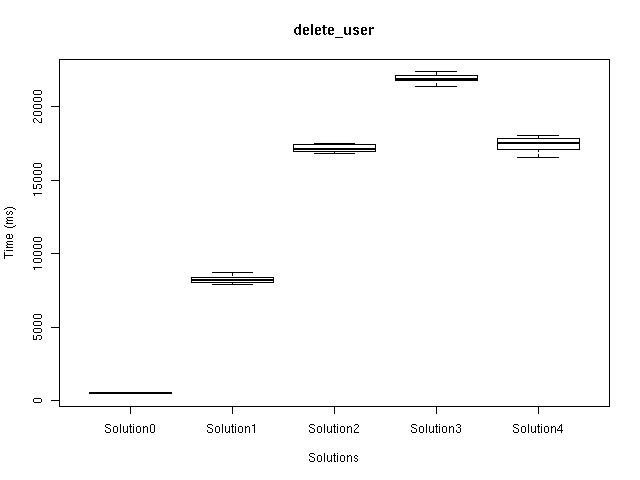
\includegraphics[width=\Width]{./figure/result/bp-delete_user.png}
	} 
	\subfigure[Enrolment]{
	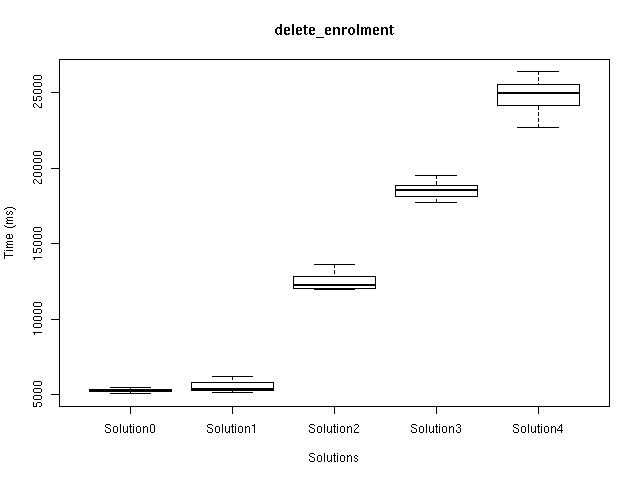
\includegraphics[width=\Width]{./figure/result/bp-delete_enrolment.png}
	}
	\caption{Delete}
\end{figure}



\newcommand{\B}[1]{\colorbox{light-gray}{#1}} %
\begin{table} 
\centering
\caption{Average time and Standard Deviation}
\begin{tabular}{ccc cccc}
\toprule
&&Solution0 & Solution1 & Solution2 & Solution3 & Solution4\\
% && $\bar{x} \; (\sigma)$ & $\bar{x} \sigma$ & $\bar{x} \sigma$ & $\bar{x}\sigma$\\
\midrule
\multirow{3}{*}{insert} & u & 0.624 (0.138) & \B{ 0.614 (0.029)} & 1.140 (0.057)
& 3.444 (0.070) & 0.586 (0.039)\\
 & c & 0.630 (0.069) & 0.621 (0.027) & 1.181 (0.087) & 3.447 (0.096) & 0.584 (0.030)\\
 & e & 5.708 (0.310) & 16.883 (0.278) & 34.220 (1.399) & 55.359 (0.351) & 15.340 (0.276)\\
\midrule
\multirow{3}{*}{update} & u & 1.254 (0.051) & 32.312 (1.207) & 25.046 (0.986) & 113.579 (1.495) & 48.000 (1.537)\\
 & c & 1.376 (0.099) & 7.559 (0.297) & 10.885 (0.384) & 19.279 (0.252) & 7.580 (0.288)\\
 & e & 7.237 (0.425) & 18.228 (0.276) & 35.673 (1.402) & 56.762 (0.420) & 16.694 (0.386)\\
\midrule
\multirow{3}{*}{delete} & u & 0.592 (0.022) & 10.798 (0.409) & 18.952 (0.600) & 42.544 (0.619) & 35.919 (0.576)\\
 & c & 0.627 (0.023) & 3.602 (0.092) & 4.828 (0.118) & 6.745 (0.120) & 3.324 (0.079)\\
 & e & 5.847 (0.294) & 5.904 (0.359) & 12.282 (0.650) & 35.070 (0.472) & 5.879 (0.240)\\
\bottomrule
\end{tabular}

 \centering
\caption{Ratio}\label{t:}
\begin{tabular}{ccccccc}
\toprule
&&Solution0 & Solution1 & Solution2 & Solution3 & Solution4\\
\midrule
\multirow{3}{*}{insert} & u & 0.624 & 0.984 & 1.826 & 5.520 & 0.938\\
 & c & 0.630 & 0.985 & 1.874 & 5.471 & 0.927\\
 & e & 5.708 & 2.958 & 5.996 & 9.699 & 2.688\\
\midrule
\multirow{3}{*}{update} & u & 1.254 & 25.761 & 19.968 & 90.553 & 38.269\\
 & c & 1.376 & 5.492 & 7.908 & 14.006 & 5.507\\
 & e & 7.237 & 2.519 & 4.929 & 7.843 & 2.307\\
\midrule
\multirow{3}{*}{delete} & u & 0.592 & 18.243 & 32.019 & 71.877 & 60.685\\
 & c & 0.627 & 5.744 & 7.700 & 10.758 & 5.302\\
 & e & 5.847 & 1.010 & 2.101 & 5.998 & 1.005\\
\bottomrule
\end{tabular}
\end{table}

\section{Analysis of results}



